
\documentclass[finnish, 12pt, a4paper, elec, utf8, a-1b, online]{aaltothesis}

\usepackage{graphicx}
\usepackage{epstopdf}
\usepackage{natbib}
\usepackage{amsfonts}
\usepackage{amssymb}
\usepackage{amsmath}

\university{Aalto-yliopisto}
\school{Sähkötekniikan korkeakoulu}

\degreeprogram{Sähkötekniikan kandidaattiohjelma}

\major{Bioinformaatioteknologia}

\code{ELEC3016}

\univdegree{BSc}

\thesisauthor{Joonas Laitinen}
%%
\thesistitle{EEG/MEG-mittausdatan analyysi aika- ja taajuusalueella MUSIC-algoritmilla}

\place{Espoo}
 
\date{15.9.2018}

\supervisor{TkT Markus Turunen}

\advisor{Prof.\ Jukka Sarvas}

\uselogo{aaltoRed}{!}

\keywords{MEG, EEG, MUSIC}

\thesisabstract{
Tähän tulee kirjoittaa tiivistelmä, että se jää osaksi PDF:n metadataa. Tämän sisältö siirtyy automaattisesti tiivistelmän osioon.
}

\copyrighttext{Copyright \noexpand\copyright\ \number\year\ \ThesisAuthor}
{Copyright \copyright{} \number\year{} \ThesisAuthor}


\begin{document}
	
\makecoverpage{}

\begin{abstractpage}[finnish]
	\abstracttext{}
\end{abstractpage}

\newpage

%% Sisällysluettelo
\thesistableofcontents

\clearpage

\section{Johdanto (tulee vielä muuttumaan)}
Aivojen toiminta perustuu sähkökemiallisiin vuorovaikutuksiin hermosolujen eli neuronien kautta. Kynnyksen ylittävä ärsyke saa aikaan hermoimpulssin, joka kulkee hermosolua pitkin ja signaali välittyy neuronilta toiselle synapsin kautta.\cite{} 
Elektroenkefalografian (EEG) avulla saadaan mitattua aivojen potentiaalierojen vaihtelua hyvällä aikaresoluutiolla. EEG:tä käytetään usein epilepsian toteamiseen sekä unen analyysiin. \cite{Nunez2006ElectricEEG}

Neuronien tuottamat sähkövirrat saavat aikaan ympärilleen heikkoja magneettikenttiä, jotka voidaan mitata pään ulkopuolelta magnetoenkefalografialla (MEG) \cite{Hamalainen1993MagnetoencephalographytheoryBrain}. MEG-laitteessa käytetään suprajohtavia SQUID-antureita. 

EEG:n ja MEG:n avulla saadaan tietoa aivojen aktiivisuudesta, mutta usean signaalilähteen yhtäaikainen toiminta aiheuttaa hankaluuksia paikantaa tietty lähde. Monenlaisia menetelmiä lähteen paikantamiselle on keksitty,joista yksi merkittävimmistä on MUSIC-algoritmi (Multiple Signal Classification), joka perustuu mittausdatan aliavaruuksien käyttöön. MUSIC-algoritmilla pystytään mittaamaan useita signaaleja yhtäaikaisesti suurella resoluutiolla. \cite{Mosher1999SourceMUSIC}

Tämän kandidaattityön tarkoituksena on selvittää, miten MUSIC-algoritmilla saadaan paikannettua signaalin lähteitä EEG- ja MEG-datan analyysissä. Mittausdataa kerätään sekä aika- että taajuusalueella ja analysoidaan MUSIC-algoritmilla MATLAB-ohjelman avulla. Työssä perehdytään myös MUSIC-algoritmin iteratiivisiin menetelmiin, RAP- sekä TRAP-MUSIC -algoritmeihin.


\clearpage
\subsection{MUSIC-algoritmi}
\cite{Schmidt1986MultipleEstimation} kehitti MUSIC-algoritmin (Multiple Signal Classification), joka perustuu mittausdatan jakamiseen keskenään ortogonaalisiin signaali- ja kohina-aliavaruuksiin, jonka jälkeen tarkistetaan potentiaalisen lähdepisteen topografian kuuluminen signaaliavaruuteen \citep{Mosher1999SourceMUSIC}. Algoritmissa lähteet kuvataan sähköisinä dipoleina ja se vaatii päämalliin tehdyn "forward modelin" (suomennos?).

Dipolit aivoissa voidaan olettaa kiinnitetyiksi eli niiden sijainnit eivät muutu ajan suhteen. MUSIC-algoritmit voidaan jakaa kahteen kategoriaan riippuen, miten dipolien suuntautumiset oletetaan olevan. Dipolit voivat olla joko kiinteästi suuntautuneita eli niiden suuntautuminen tiedetään etukäteen tai vapaasti suuntautuvia, jolloin niiden suuntausta ei tiedetä. \citep{Makela2018TruncatedLocalization} 

\subsubsection{Skalaari-MUSIC}
Aloitetaan esittelemällä kiinnitetyn orientaation MUSIC-algoritmi, jota kutsutaan myös skalaari-MUSIC-algoritmiksi. Olkoon pisteessä $\mathbf{p}$ dipoli, jolla on orientaatio $\eta$. Olkoon mittauksista saatu data kerättynä matriisiin $\mathbf{Y}\in \mathbb{R}^{m\times N}$, jossa $\mathit{m}$ on mittaussensorien määrä ja $\mathit{N}$ mittausten lukumäärä. Sensorit mittaavat dipolien topografiaa $\mathbf{l(p,\eta)}$. Matriisilla $\mathbf{Y}$ on muoto

\begin{equation}
    \mathbf{Y=AS+\epsilon},
\end{equation}
jossa $\mathbf{A =[l(p}_1,\eta_1),...,\mathbf{l(p}_n,\eta_n)]$ on sekoitusmatriisi, $\mathbf{S}$ ajankulkumatriisi ja $\mathbf{\epsilon}$ mittauskohinaa. Lähteen orientaatio on kiinnitetyn orientaation tapauksessa riippuvainen vain sen sijainnista eli $\mathbf{l(p},\eta)=\mathbf{L(p})\mathbf{\eta}(\mathbf{p})$, jossa $\mathbf{L(p) = [l(p,e_x),l(p,e_y),l(p,e_z)]}$ on "lead-field-matriisi", joka sisältää pisteen $\mathbf{p}$ topografiat jokaisen karteesisen koordinaatin suunnassa. 

Data-avaruus $\text{span}(\mathbf{Y})$ jaetaan keskenään ortogonaalisiin aliavaruuksiin, signaali-avaruuteen $\text{span}(\mathbf{A})$  ja kohina-avaruuteen $\text{span}(\mathbf{A^\bot})$  \citep{Mosher1999SourceMUSIC}. Ortogonaaliprojektio signaaliavaruuteen $\text{span}(\mathbf{A})$ voidaan approksimoida kaavan (\ref{eq:6}) avulla

\begin{equation}
    \mathbf{P}_{sg}=\mathbf{U}(:,1:n)\mathbf{U}(:,1:n)^T,
\end{equation}
jossa $\mathbf{U}$ on ortogonaalinen matriisi singulaariarvohajotelmasta ja $\mathit{n}$ on lähteiden määrä. 

Yleensä lähteiden määrää ei tiedetä, joten se täytyy approksimoida. Datamatriisin ominaisarvoista voidaan päätellä, kuinka monta voimakasta lähdettä löydetään. Ominaisarvoista voidaan muodostaa pylväsdiagrammi ja lähteiden määrä voidaan approksimoida sen mukaan, missä kohdassa tapahtuu merkittävä pudotus. Valkoisen kohinan tapauksessa pylväät tasoittuvat loppupäässä, kun lähteet ovat loppuneet. Värillisellä kohinalla pudotuksen löytäminen on hankalampaa ja täten lähteiden approksimaatio on vaikeampaa. Kuvassa \ref{fig:D} on simuloidun mittausdatan ominaisarvot pylväsdiagrammeina valkoisen ja värillisen kohinan tapauksissa.

Olkoon approksimoitujen lähteiden määrä \~{n}. Projektio voidaan nyt muodostaa approksimoitujen lähteiden määrän mukaan $\mathbf{P}_{s}=\mathbf{U}(:,1:\~n)\mathbf{U}(:,1:\~n)^T$, jolloin \~n jälkeiset ominaisvektorit kuvaavat pelkkää kohinaa.

\clearpage
\begin{figure}[ht]
    \centering
    \begin{minipage}{0.45\textwidth}
        \centering
        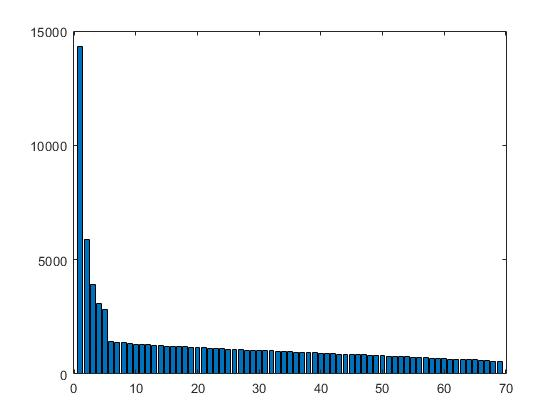
\includegraphics[width=1\textwidth]{d_valk.jpg} % first figure itself
    \end{minipage}\hfill
    \begin{minipage}{0.45\textwidth}
        \centering
        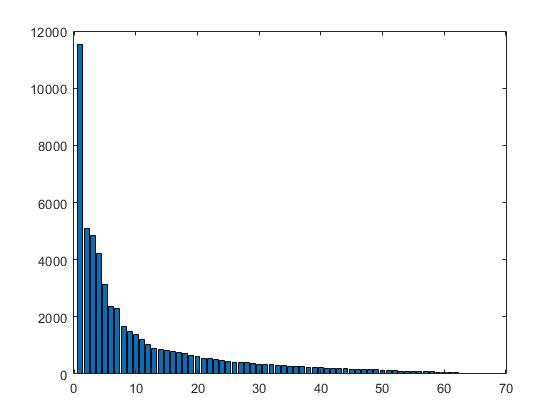
\includegraphics[width=1\textwidth]{d_var.jpg} % second figure itself
    \end{minipage}
    \caption{Vasemman puoleisessa kuvassa simuloitu data sisältää valkoista kohinaa ja oikean puoleisessa kuvassa värillistä kohinaa. Molemmissa simulaatioissa on viisi lähdettä ja kohinan määrä on yhtä suuri.}
    \label{fig:D}
\end{figure}

Pisteen $\mathbf{p}$ kuuluminen signaaliavaruuteen tarkistetaan projektio-operaattorin avulla. Pisteen $\mathbf{p}$ topografia $\mathbf{l(p)}$ lasketaan "forward modelin avulla. Topografia kuuluu signaaliavaruuteen, jos sen projektio signaaliavaruuteen on topografia itse. Toisin sanoen piste $\mathbf{p}$ on lähde, jos $\mathbf{P}_s\mathbf{l(p)} = \mathbf{l(p)}$. Tämä tarkoittaa sitä, että jos $\mathbf{l(p)}$ sijaitsee signaaliavaruudessa, sen normi ei muutu projektiossa eli $||\mathbf{P}_s\mathbf{l(p)}||=||\mathbf{l(p)}||$. Jos $\mathbf{l(p)}$ ei sijaitse signaaliavaruudessa, niin sen projektion normi on pienempi kuin $\mathbf{l(p)}$:n normi eli
$||\mathbf{P}_s\mathbf{l(p)}||<||\mathbf{l(p)}||$.

Näistä saadaan muodostettua paikannusfunktio, joka laskee jokaisen pisteen $\mathbf{p}$ kuulumisen signaaliavaruuteen

\begin{equation}
    \mathbf{\mu(p)} = \frac{||\mathbf{P}_s\mathbf{l(p)}||^2}{||\mathbf{l(p)}||^2} 
    \begin{cases}
    =1\text{, jos p on lähde}\\
    <1\text{, jos p ei ole lähde}
     \end{cases}
\end{equation}

\subsubsection{Vektori-MUSIC}
Vapaan orientaation tapauksessa jokaiselle pisteelle $\mathbf{p}$ määräytyy suuntaus $\mathbf{\eta}$ mittausdatan perusteella. Vapaan orientaation MUSIC-algoritmia kutsutaan myös vektori-MUSIC -algoritmiksi. Vektori-MUSIC -algoritmi muodostetaan hyvin samalla tavalla kuin skalaari-MUSIC, mutta sen paikannusfunktio muodostetaan eri tavalla

\begin{equation}
    \mathbf{\mu(p)} = \max_{||\eta||=1} \frac{||\mathbf{P}_s\mathbf{L(p)\eta}||^2}{||\mathbf{L(p)\eta}||^2}
\end{equation}

(jatkuu kunhan opin selittämään)

\clearpage
\begin{figure}[h!]
    \centering
    \begin{minipage}{0.45\textwidth}
        \centering
        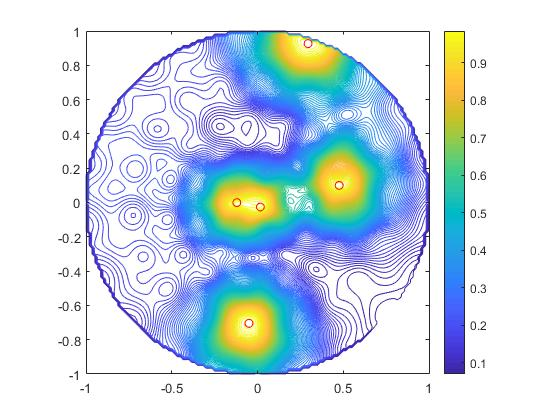
\includegraphics[width=1\textwidth]{MUSICfix.jpg}
    \end{minipage}\hfill
    \begin{minipage}{0.45\textwidth}
        \centering
        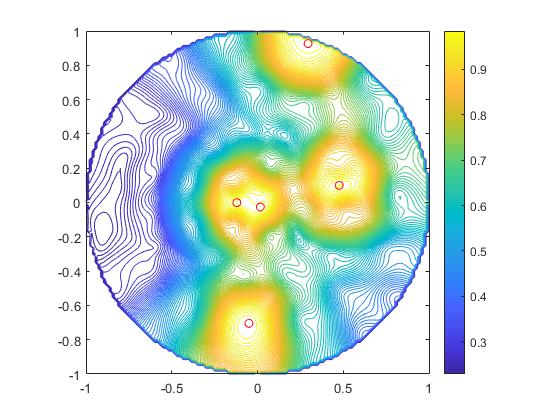
\includegraphics[width=1\textwidth]{MUSICfree.jpg} 
    \end{minipage}
    \caption{MUSIC-algoritmin simuloiminen pallomallin avulla MATLAB-ohjelmalla. Punaiset pisteet ovat sattumanvaraisesti sijoitettuja lähteitä ja topografia on tehty MUSIC-algoritmin avulla. Vasemmanpuoleisessa kuvassa on käytetty fixed-orientationia ja oikeanpuoleisessa free-orientationia. Molemmissa tapauksissa kohina on valkoista.}
    \label{fig:MUSIC}
\end{figure}

Kuvasta \ref{fig:MUSIC} huomataan, että MUSIC vapaalla orientaatiolla saa aikaan suurempia aktiivisuuden alueita, mikä vaikeuttaa lähteiden paikantamista.
\section{Mittausdatan analyysi MUSIC-algoritmilla}
\section{Tulokset}
\section{Yhteenveto}
\clearpage


\bibliographystyle{agsm}    % Käytettävä viittausjärjestelmä, agsm = harvard
\bibliography{Lahteet}      % BibTeX-tietokanta, lahteet tiedoston nimi

\end{document}
